
\section{Введение и краткая теория}

Интерферометр Майкельсона находит применение в спектрометрах с высоким разрешением, для абсолютных и относительных измерений длин с точностью 0,005 мкм. 

Оптическая схема интерферометра приведена на рис. 1. Источником света служит лазер $ЛГ$. Лазер излучает узкий пучок света, который фокусируется линзой Л1. В фокусе этой линзы возникает точечный
источник света S. Сферическая световая волна от источника S падает на делительный кубик ДК и делится его диагональной гранью на 
две волны — отражённую $1$ и проходящую $2$. Волна 1 отражается от
зеркала $З_1$, возвращается к кубику, частично проходит сквозь него и
попадает на экран $Э$. Волна $2$ отражается от зеркала $З_2$, частично отражается от кубика и также попадает на экран. Световые волны $1$ и $2$
испускаются одним источником S, и они когерентны между собой. Эти
волны создают на экране $Э$ интерференционную картину. Для увеличения масштаба интерференционной картины может быть использована
линза $Л_2$.

Зеркало З1 установлено перпендикулярно падающему лучу. Оно может перемещаться вдоль луча. Это зеркало в дальнейшем будет называться подвижным. Зеркало З2 вдоль направления падающего луча не
перемещается. Его, однако, можно наклонять по отношению к лучу.

\begin{figure}[h!]
    \centering
    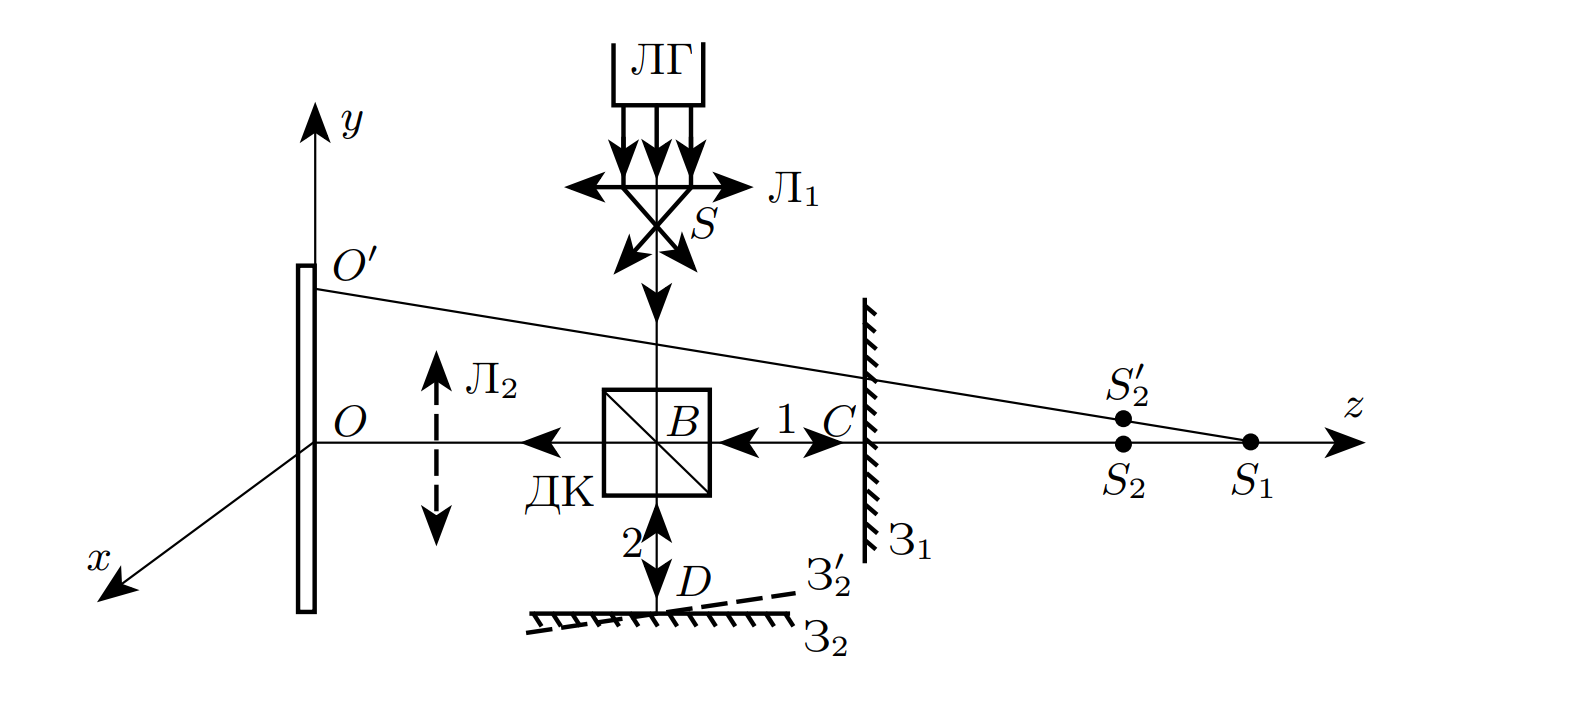
\includegraphics[width=1.2\linewidth]{pics/scheme.png}
    \caption{Схема интерферометра}
    \label{}
\end{figure}

